\chapter{Ensayos y Resultados}
\label{Chapter4}

Para la validación del prototipo se realizaron distintas pruebas en hardware y el software a fin de cubrir los requerimientos explicados en \ref{subsec:Requerimientos}. Aquí se desarrollan las resultados para ambos partes de manera separada.

\section{ Pruebas funcionales del software }
\label{sec:pruebasSW}

El firmware esta basado en módulos propios mas módulos de terceros de los cuales en la figura \ref{fig:diag_Repositorio} se muestra la vinculación de los mismos e inclusión de rutinas en cada uno. Cabe mencionar que la estructura del proyecto se basa en el repositorio utilizado en la materia de \textit{Sistemas Operativos de Tiempo Real} \citep{ws_ridolfi}.   
% Figura con arbol de directorios del proyecto
\begin{figure}[h!]
	\centering
	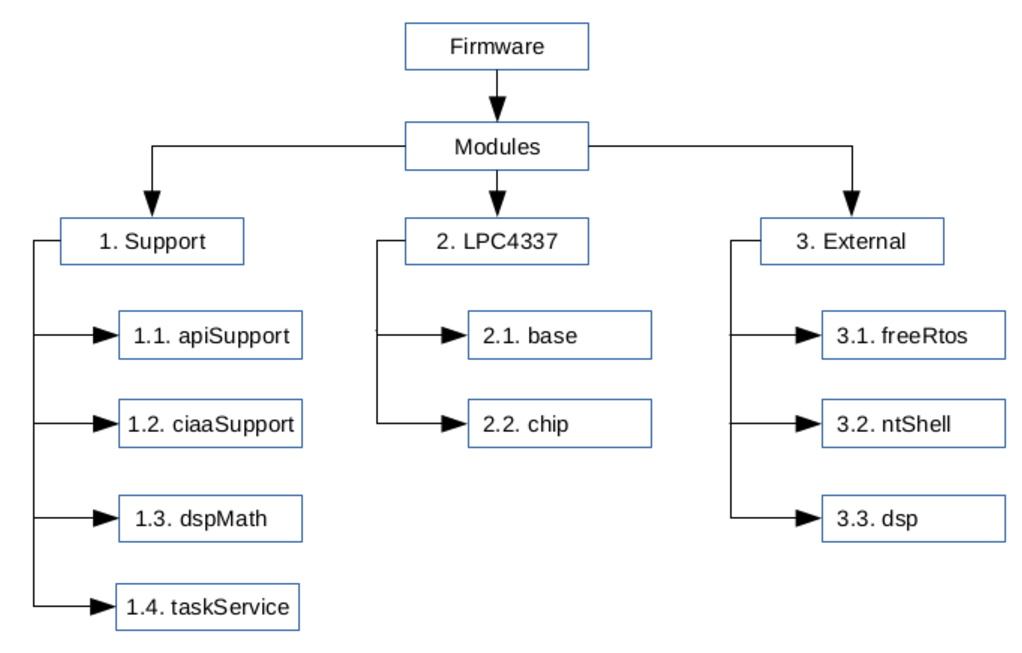
\includegraphics[width=1.0\textwidth]{Figures/Cap_4/diagrama_repositorio}
	\caption{Estructura de directorios del proyecto.}
	\label{fig:diag_Repositorio}
\end{figure}

En la estructura de directorios \textit{support} se encuentran los  de desarrollo propio. Dentro de los directorios \textit{LPC4337} se encuentran los módulos de capa HAL y los CMSIS \ref{ agregar referencia }. En la ubicación \textit{Extrernal} se encuentran los módulos con  de soporte de terceros.


\subsection{ Pruebas unitarias }

Se realizaron sobre los módulos propios ubicados en el directorio \textit{Support} del repositorio. Los mismos interactúan entre los servicios de la aplicación y las rutinas de capa HAL \footnotemark. Sobre la capa HAL y los librerías de terceros no se realizaron pruebas, se confió en el funcionamientos de los mismos.

A fin de validar el comportamiento de los algoritmos de procesamiento de los sensores de temperatura se realizaron pruebas sobre archivos con datos de entradas y se generaron archivos de salida con los resultados obtenidos. En la figura \ref{fig:diag_test_temp} se observa los tipos de archivos que se procesan.
% RESULTADOS DE LOS TEST DE TEMPERATURA
\begin{figure}[h!]
	\centering
	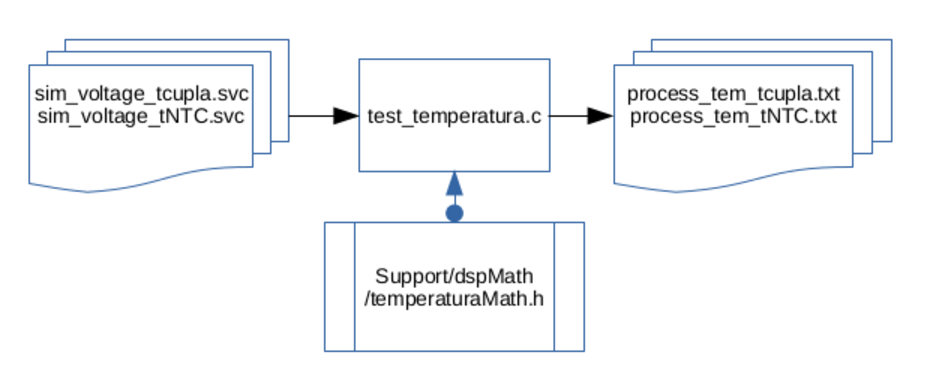
\includegraphics[width=1.0\textwidth]{Figures/Cap_4/diag_test_temperatura}
	\caption{Test de funciones interfaz de temperatura.}
	\label{fig:diag_test_temp}
\end{figure}

\footnotetext{HAL: hardware abstraction level}

La escritura en memoria interna se probó un procedimiento de emulación de datos con archivos de texto plano de entrada y salida,  validando la escritura de bloques binarios según los formatos establecidos en la lógica del programa. En la figura \ref{fig:diag_test_mem} se observa los archivos procesados en el test.
%RESULTADOS DE LOS TEST DE ESCRITURA EN MEMORIA
\begin{figure}[h!]
	\centering
	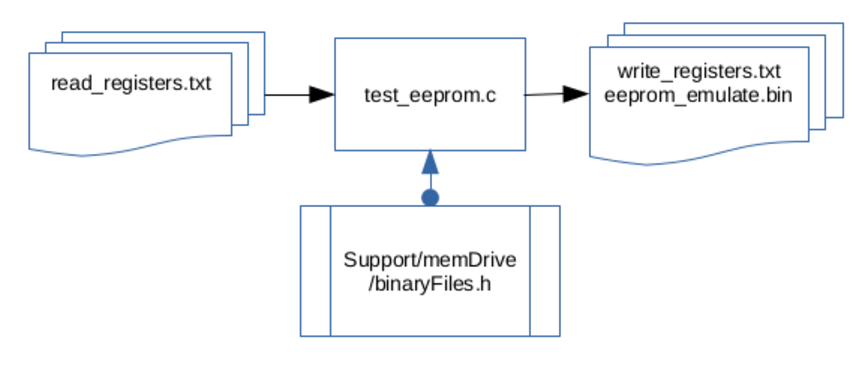
\includegraphics[width=0.9\textwidth]{Figures/Cap_4/diag_test_memoria}
	\caption{Test de funciones interfaz de memoria.}
	\label{fig:diag_test_mem}
\end{figure}

Para estas pruebas se predefinieron los archivos de ingreso de datos de manera de simplificar la lectura de los bloques de información. En las figuras \ref{fig:files_test_mem} y \ref{fig:files_test_temp} se observan la estructura de los archivos procesados.

\begin{figure}[h!]
	\centering
	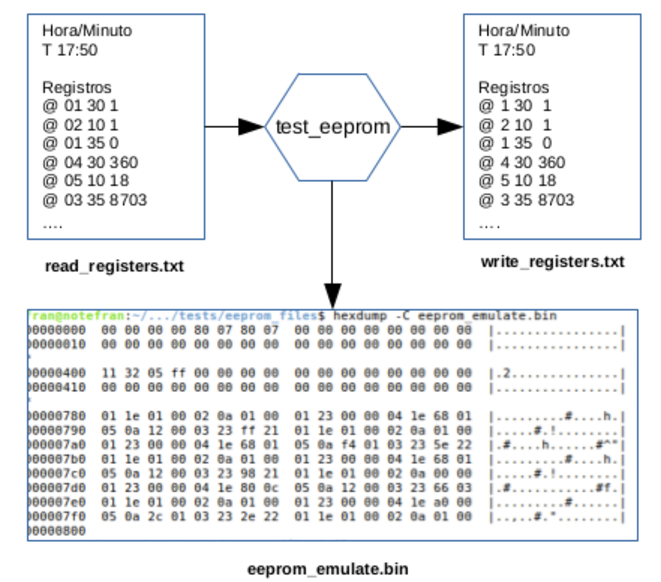
\includegraphics[width=0.9\textwidth]{Figures/Cap_4/files_test_temperatura}
	\caption{ Archivos procesados en el test de temperatura.}
	\label{fig:files_test_temp}
\end{figure}

\begin{figure}[h!]
	\centering
	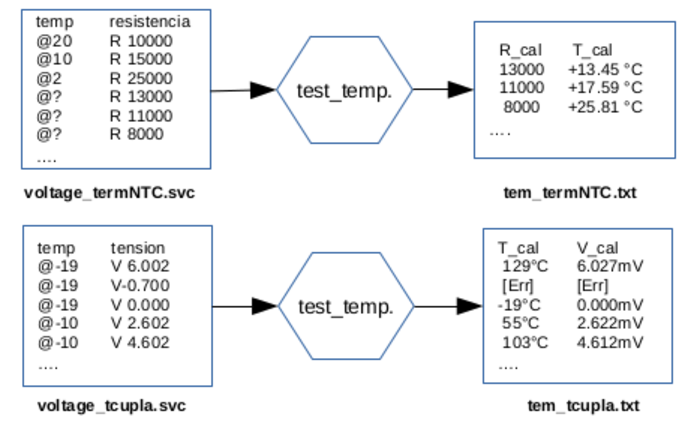
\includegraphics[width=0.9\textwidth]{Figures/Cap_4/files_test_memoria}
	\caption{Archivos procesados en el test de memoria.}
	\label{fig:files_test_mem}
\end{figure}


\subsection{ Pruebas de Integración }

Se probó el funcionamiento de los comandos vía consola y su impacto sobre las configuraciones de los puertos y la devolución de estados por pantalla. 

% figuras de modificion de estructuras y pantalla?
\begin{figure}[h!]
	\centering
	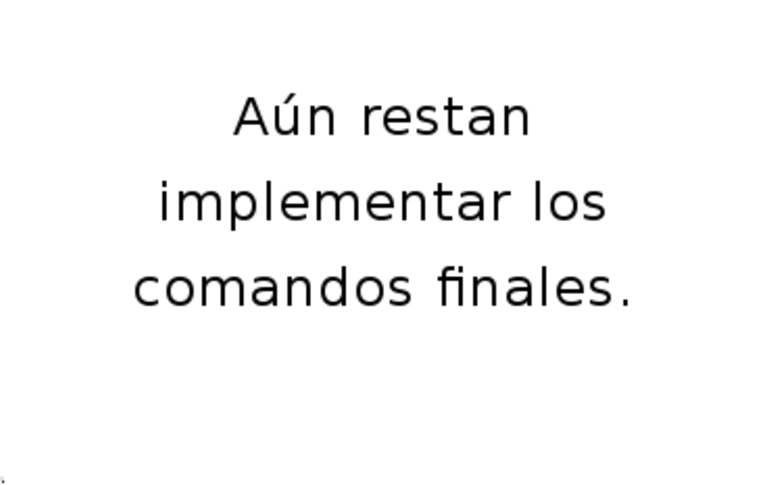
\includegraphics[width=1.0\textwidth]{Figures/Cap_4/imagen_mensaje}
	\caption{Respuesta a un comando de configuración.}
	\label{fig:term_Configuracion}
\end{figure}

Se probó la estabilidad del mismo dejando en funcionamiento durante un día completo, de esta manera se tiene mejor información de la perfomance de tiempo de uso y memoria de los servicios en el sistema operativo. En la tabla \ref{tabla_rendimiento} se observa el resultado obtenido en uso de memoria y tiempo de CPU.

% Tabla con los valores de rendimiento
\begin{table}[h!]
\centering
\begin{tabular}{ m{1.0cm}|m{3.0cm}|m{2.0cm}|m{2.5cm} }\hline
{\textbf{Id}} &{\textbf{Nombre}} & {\textbf{CPU(\%)}} & {\textbf{Memoria(Byte)}}\\ \hline
{0} & {Task Idle} & { 95 } & { 128 }\\ \hline
{1} & {Task Outputs} & { 1 } & { 256 }\\ \hline
{2} & {Task Inputs}  & { 1 } & { 256 }\\ \hline
{3} & {Task Terminal} & { 3 } & { 512 }\\ \hline
{4} & {Task Eeprom } & { 1 } & { 256 }\\ \hline
\end{tabular}
\caption{Uso de recursos por tarea.}
\label{tabla_rendimiento}
\end{table}

Considerando que este microprocesador (LPC-4337) tiene 32KB de memoria RAM, con mas la mitad disponible las tareas solo consumen 1408 Bytes y menos del 4\% del CPU. Por lo tanto se tienen recursos de sobra para poder seguir implementando servicios y funciones en la plataforma.

\section{ Ensayos de validación hardware }
\label{sec:pruebasHW}

Para esto se realizaron las pruebas sobre los puertos de la EDU-CIAA emulando el comportamiento de los sensores en función de los modos de funcionamiento preestablecidos. En la figura \ref{fig:foto_prototipo} se observa el banco de pruebas que emula las entradas y salidas que se tendrían en el entorno real.
% AGREGAR CAPTURAS DEL SISTEMA - BANCO DE PRUEBA CON LOS RESULTADOS.
% figuras de modificion de estructuras y pantalla?
\begin{figure}[h!]
	\centering
	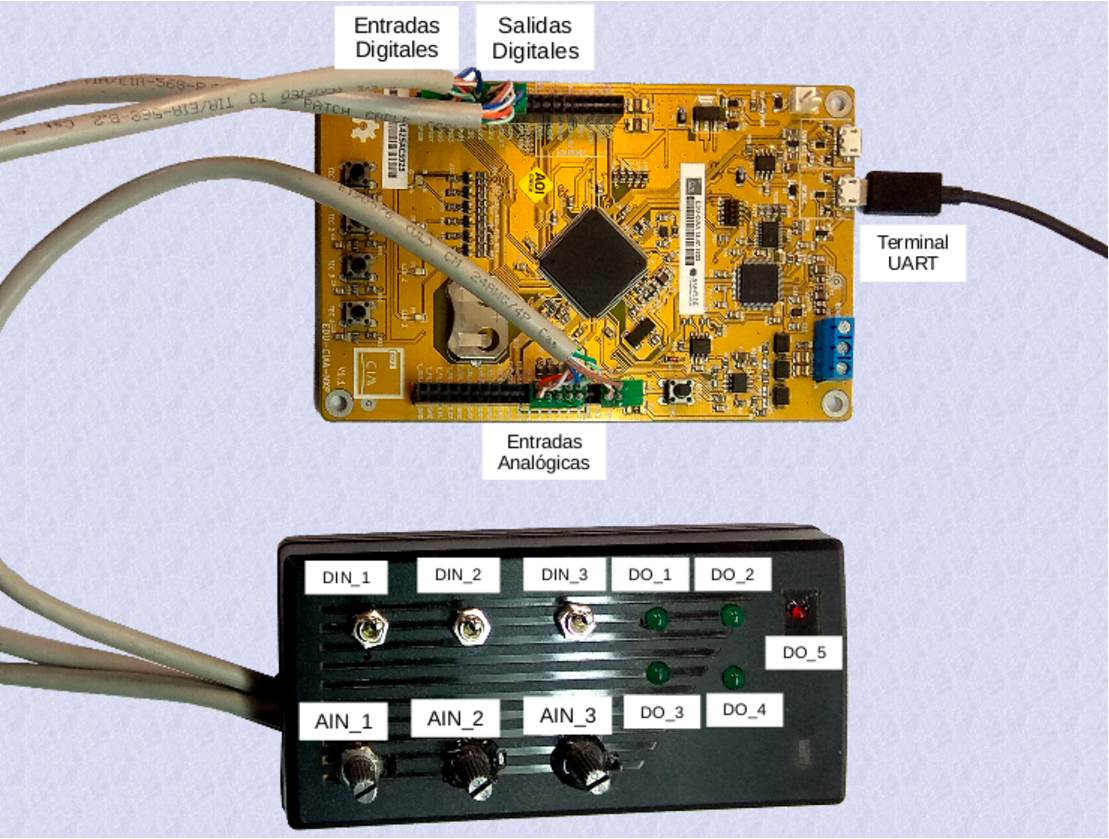
\includegraphics[width=1.0\textwidth]{Figures/Cap_4/foto_prototipo}
	\caption{Banco de pruebas.}
	\label{fig:foto_prototipo}
\end{figure}

\subsection{ Pruebas de interfaz }

Para esto simplemente se ingresaron los comandos establecidos y verificaron que los mismos ejecuten correctamente las acciones internas así también como los mensajes por la terminal.Se tomaron luego capturas de los estados de salida así como de la terminal y de log registrado por el sistema. En las figuras \ref{falta_imagen} se muestran las ejecuciones de algunos de ellos.



\subsection{ Validación de requerimientos }

Para esto se tomaron los criterios desarrollados conjuntamente con los requerimientos previamente en la materia \emph{Gestión de Proyectos} del posgrado. Básicamente consiste en variar los valores de los entradas al prototipo y verificar que cumpla con la respuesta adecuada.\\
En la tabla \ref{tablas_cumplimiento_req} se observa un resumen del cumplimiento de los requerimientos funcionales y de interfaz. Para los mismos se evaluó si cumple si o no, y en caso negativo porque no.
% tabla con los resultados de cumplimiento.
\begin{table}[h!]
\begin{flushleft}
\begin{tabular}{|m{2.6cm}|m{1.5cm}|m{1.5cm}|m{6.8cm}|}\hline
{\textbf{Requerimiento}} & {\textbf{Número}} & {\textbf{Cumple}} & {\textbf{Observaciones}}\\ \hline
\multicolumn{1}{|l|}{RFTEM} & { 1.1.1 } & { SI } & { Ninguna. }\\ \cline{ 2- 4}
\multicolumn{1}{|l|}{} & { 1.1.2 } & { SI } & { Ninguna. } \\ \cline{ 2- 4}
\multicolumn{1}{|l|}{} & { 1.1.3 } & { SI } & { Ninguna. } \\ \cline{ 2- 4}
\multicolumn{1}{|l|}{} & { 1.1.4 } & { SI } & { Ninguna. } \\ \cline{ 2- 4}
\multicolumn{1}{|l|}{} & { 1.1.5 } & { SI } & { Ninguna. } \\ \cline{ 2- 4}
\multicolumn{1}{|l|}{} & { 1.1.6 } & { NO } & { Memoria interna insuficiente. } \\ \hline
\multicolumn{1}{|l|}{RFENE} & { 1.2.1 } & { SI } & { Ninguna. }\\ \cline{ 2- 4} 
\multicolumn{1}{|l|}{} & { 1.2.2 } & { NO } & { Se supone constante 5V. } \\ \cline{ 2- 4}
\multicolumn{1}{|l|}{} & { 1.2.3 } & { NO } & { Memoria interna insuficiente. } \\ \cline{ 2- 4}
\multicolumn{1}{|l|}{} & { 1.2.4 } & { SI } & { Por ahora solo se pueden ingresar comandos. } \\ \hline
\multicolumn{1}{|l|}{RFCOND} & { 1.3.1 } & { SI } & { Ninguna. }\\ \cline{ 2- 4} 
\multicolumn{1}{|l|}{} & { 1.3.2 } & { SI } & { Ninguna. }\\ \hline
\multicolumn{1}{|l|}{RFTI} & { 1.4.1 } & { NO } & { No implementado sistema distribuido. }\\ \cline{ 2- 4} 
\multicolumn{1}{|l|}{} & { 1.4.2 } & { SI } & { Ninguna. }\\ \cline{ 2- 4} 
\multicolumn{1}{|l|}{} & { 1.2.3 } & { NO } & { No implementado sistema distribuido. }\\ \hline
\multicolumn{1}{|l|}{RFNB} & { 1.5.1 } & { SI } & { Ninguna. }\\ \cline{ 2- 4} 
\multicolumn{1}{|l|}{} & { 1.5.2 } & { SI } & { Ninguna. }\\ \hline
\multicolumn{1}{|l|}{RFHMI} & { 1.6.1 } & { SI } & { Ninguna. }\\ \cline{ 2- 4} 
\multicolumn{1}{|l|}{} & { 1.6.2 } & { NO } & { No implementado sistema distribuido. }\\ \cline{ 2- 4} 
\multicolumn{1}{|l|}{} & { 1.6.3 } & { SI } & { Ninguna. }\\ \cline{ 2- 4} 
\multicolumn{1}{|l|}{} & { 1.6.4 } & { NO } & { No implementado sistema distribuido. }\\ \cline{ 2- 4} 
\multicolumn{1}{|l|}{} & { 1.6.5 } & { NO } & { No implementado sistema distribuido. }\\ \hline 
\multicolumn{1}{|l|}{RITEM} & { 2.1.1 } & { SI } & { Ver sección \ref{analisis_hardware}. }\\ \cline{ 2- 4} 
\multicolumn{1}{|l|}{} & { 2.1.2 } & { SI } & { Ver sección \ref{analisis_hardware}. }\\ \hline 
\multicolumn{1}{|l|}{RIENE} & { 2.2.1 } & { SI } & { Ninguna. }\\ \cline{ 2- 4} 
\multicolumn{1}{|l|}{} & { 2.2.2 } & { NO } & { Se supone parámetro constante 5V. }\\ \hline
\multicolumn{1}{|l|}{RICOND} & { 2.3.1 } & { SI } & { Ninguna. }\\ \cline{ 2- 4} 
\multicolumn{1}{|l|}{} & { 2.3.2 } & { SI } & { Ninguna. }\\ \hline
\multicolumn{1}{|l|}{RINB} & { 2.4.1 } & { SI } & { Ninguna. }\\ \hline
\multicolumn{1}{|l|}{RIHMI} & { 2.5.1 } & { SI } & { Ninguna. }\\ \cline{ 2- 4} 
\multicolumn{1}{|l|}{} & { 2.5.2 } & { SI } & { Solo con comandos. }\\ \cline{ 2- 4} 
\multicolumn{1}{|l|}{} & { 2.5.3 } & { SI } & { Ninguna. }\\ \cline{ 2- 4} 
\multicolumn{1}{|l|}{} & { 2.5.4 } & { SI } & { Ninguna. }\\ \cline{ 2- 4} 
\multicolumn{1}{|l|}{} & { 2.5.5 } & { SI } & { Ninguna. }\\ \cline{ 2- 4} 
\multicolumn{1}{|l|}{} & { 2.5.6 } & { NO } & { Se puede implementar en la misma plataforma a futuro. }\\ \hline
\multicolumn{1}{|l|}{RNF} & { 3.1 } & { NO } & { No se construyó banco de pruebas. }\\ \hline 
\multicolumn{1}{|l|}{RD} & { 4.1 } & { SI } & { Ver sección \ref{analisis_hardware}.}\\ \hline 
\end{tabular}
\end{flushleft}
\caption{ Cumplimiento de los requerimientos.}
\label{tablas_cumplimiento_req}
\end{table}

Los requerimientos a Futuro (RAF) no se han agregado a la tabla pero fueron considerados durante el desarrollo del prototipo como un sistema distribuido. En principio esa opción fue descartada y dejada para mas adelante en función de los resultados obtenidos con este primer diseño.
Muchos de los requerimientos originales estaban asociados a realizar un sistema distribuido de control con módulos de entradas y salidas conectados vía RS485 a la EDU-CIAA. Si bien ese proyecto fue modificado por el actual los requerimiento se conservaron a modo demostrativo de como se transformó desde la idea inicial.